\setchapterpreamble[u]{\margintoc}

\chapter{Grupos de homología relativa}
Como vinos en el capítulo anterior, el grupo de homología de orden $1$ de la
rosa tiene un generador por cada pétalo. Esto parece decirnos que la acción
de \emph{añadir un pétalo} (\textbf{adjunción}) provoca la aparición de
nuevos generadores. No obstante, diferentes adjunciones provocan diferentes
alteraciones:

\begin{itemize}
\item Si pegamos sólo uno de los extremos del segmento a $B_p$ y dejamos el
otro libre, $B_p$ es un retracto por deformación fuerte de la figura
resultante, de forma que no aparecen nuevos generadores.
\item Si lo pegamos por ambos lados, aparece un pétalo nuevo y un nuevo
generador.
\end{itemize}

Dado un espacio topológico $X$ y un subespacio $A \subseteq X$, el grupo de
homología relativa estudia cómo $A$ está pegado con su complementario,
$X\backslash A$. Diremos que dos cadenas son \textit{iguales módulo $A$} si
su diferencia es una cadena en $A$. En particular, tendremos que una cadena
será un \textit{ciclo módulo $A$} si su borde está contenido en $A$.

\section{Complejo de cadenas cociente}
\begin{definition}
Sea $(C,\partial)$ un complejo de cadenas y $(D,\partial')$ un subcomplejo de
cadenas, con $D$ subgrupo normal de $C$. Se define el \textbf{complejo
cociente} como el grupo graduado $C/D$ dotado del operador borde
\begin{diag}
\frac{C_p}{D_p} \arrow[r]& \frac{C_{p-1}}{D_{p-1}}\\[-8mm]
\overline c \arrow[r, maps to] & \overline{\p c}
\end{diag}
\end{definition}

Si $\pi\colon C \to C/D$ es el epimorfismo canónico e $i\colon D
\hookrightarrow C$ es la inclusión, la sucesión
\[0 \longrightarrow D \xrightarrow{i} C \xrightarrow{\pi} \frac{C}{D}
\longrightarrow 0\]
es exacta. Según el \refthm{SucExacHomo}, si podemos hallar un
homomorfismo de conexión $\Delta\colon H_*(C/D) \to H_*(C)$, la sucesión
\begin{equation}
\label{SECociente}
H_*(D) \xrightarrow{i_*} H_*(C) \xrightarrow{\pi_*}
H_*(C/D) \xrightarrow{\Delta} H_*(D)
\end{equation}
será exacta.

Para construir el homomorfismo de conexión, sea $\overline c \in Z_n(C/D)$.
Tenemos que
\[\overline{\p c}=0 \implies \partial c \in D_{n-1}\]
Como $\p^2c=0$, $\p c \in Z_{n-1}(D)$, luego $[\partial c] \in H_{n-1}(D)$.
Definimos entonces el homomorfismo $\Delta_n\colon H_n(C/D) \to H_{n-1}(D)$
como
\[\Delta_n(\overline c)=[\p c]\]
de forma que $\Delta=\{\Delta_n: n \in \mb{Z}\}$ es un homomorfismo de
conexión.

\begin{lemma}[Teorema de isomorfia para grupos graduados]\lablemma{TTIGG}
Sea $C$ un complejo de cadenas y $E,D$ subcomplejos normales de $C$. Si $E$
es un subcomplejo de $D$,
\[\frac{C}{D} \cong \frac{C/E}{D/E}\]
\end{lemma}

\marginnote[-2.2cm]{
\begin{kaobox}[frametitle=Tercer teorema de isomorfía]
Sea $C$ un grupo y $D,E$ subgrupos normales de $C$. Si $E \leq D$, $E$ es
un subgrupo normal de $D$ y
\[\frac{C}{D}\cong\frac{C/E}{D/E}\]
\end{kaobox}
}

\begin{proof}
Sea $p \in \mb{Z}$. Por definición de subcomplejo y subcomplejo normal,
$D_p,E_p \trianglelefteq C_p$ y $E_p \leq D_p$. Por el tercer teorema de
isomorfia, existe un isomorfismo
\[f_p\colon \frac{C_p}{D_p} \longrightarrow \frac{C_p/E_p}{D_p/E_p}\]

Si $f$ es un homomorfismo graduado,
\[f\colon \frac{C}{D} \longrightarrow \frac{C/E}{D/E}\]
es un isomorfismo graduado por ser una colección de isomorfismos. Por tanto,
$C/D$ es isomorfo a $(C/E)/(D/E)$.
\end{proof}

Sea $C$ un complejo de cadenas y $E \leq D$ subcomplejos normales de $C$. Por
el \reflemma{TTIGG}, existe un isomorfismo graduado $f\colon (C/E)/(D/E)
\to C/D$. Si ahora consideramos el epimorfismo canónico
\[\pi\colon C/E\longrightarrow \frac{C/E}{D/E}\]
la aplicación
\[\Pi\colon \frac{C}{E} \xrightarrow{\pi} \frac{C/E}{D/E} \xrightarrow{f}
\frac{C}{D}\]
es un epimorfismo graduado entre $C/E$ y $C/D$. De aquí se
obtiene la sucesión exacta corta
\[0 \longrightarrow \frac{D}{E} \xrightarrow{i} \frac{C}{E}
\xrightarrow{\Pi}\frac{C}{D} \longrightarrow 0\]

Sea $p\colon D \to D/E$ el epimorfismo canónico. Este homomorfismo induce un
homomorfismo de grado 0 en homología,
\[p_*\colon H_*(D) \longrightarrow H_*(D/E)\]
Si $\Delta\colon H_*(C/D) \to H_*(D)$ es el homomorfismo graduado
\eqref{SECociente},
\begin{equation}
\label{DeltaCPrima}
\Delta'\colon H_*(C/D) \xrightarrow{\Delta} H_*(D) \xrightarrow{p_*} H_*(D/E)
\end{equation}
es un homomorfismo de conexión, por lo que el \eqref{SucExacHomo} nos dice
que
\begin{equation}
\label{SECociente2}
H_n(D/E) \xrightarrow{i_*} H_n(C/E) \xrightarrow{\Pi_*} H_n(C/D)
\xrightarrow{\Delta'} H_{n-1}(D/E)
\end{equation}
es una sucesión exacta larga.

Sea $C'$ otro complejo de cadenas, con $E'\leq D'$ subcomplejos normales de
$C'$. Considérese una aplicación de cadenas $g\colon C \to C'$ tal que
$g(D) \leq D'$ y $g(E) \leq E'$. Como acabamos de ver, se puede construir
una sucesión exacta corta
\[0 \longrightarrow \frac{D'}{E'} \longrightarrow \frac{C'}{E'}
\longrightarrow \frac{C'}{D'} \longrightarrow 0\]
que induce una sucesión exacta larga en homología similar a
\eqref{SECociente2}. Dado que $g$ es una aplicación de cadenas, podemos
conectar ambas sucesiones exactas usando $g_*$:
\begin{diag}
H_n(D/E) \arrow{r}{i_*} \arrow{d}{g_*} &
H_n(C/E) \arrow{r}{\Pi_*} \arrow{d}{g_*} &
H_n(C/D) \arrow{r}{\Delta'} \arrow{d}{g_*} &
H_{n-1}(D/E) \arrow{d}{g_*}\\
H_n(D'/E') \arrow{r}{\tilde i_*} &
H_n(C'/E') \arrow{r}{\tilde\Pi_*} &
H_n(C'/D') \arrow{r}{\tilde\Delta'} &
H_{n-1}(D'/E')
\end{diag}

Por cómo está construida \eqref{SECociente2}, se puede probar que cada uno
de los cuadrados del diagrama anterior es conmutativo. Se dice entonces que
$g_*$ es una \textbf{transformación natural} o que cumple la
\textbf{hipótesis de naturalidad}.

\section{Homología singular relativa}
\begin{definition}
Un \textbf{par de espacios} es un par ordenado de la forma $(X,A)$, donde
$X$ es un espacio topológico y $A \subseteq X$.
\end{definition}

Sea $(X,A)$ un par de espacios y $n > 0$. Dado un $c \in S_n(X)$, existen
$n$-símplices singulares $\phi_1,\dots,\phi_p\colon \sigma_n \to X$ y enteros
$\mu_1,\dots,\mu_p$
\[c=\sum^p_{i=1}\mu_i\phi_i\]
Si $\phi_i(\sigma_n) \subseteq A$ para cada $i=1,\dots,p$, se tiene entonces
que $c \in S_n(A)$. De aquí se sigue que $S_n(A) \leq S_n(X)$.

Por otro lado, dado un $i=0,\dots,n$,
\[\p_{(i)} \phi(\sigma_{n-1}) \subset \phi(\sigma_n) \subset A
\implies \p_{(i)}\phi \in S_{n-1}(A)\]
por lo que $S_*(A)$ es un subcomplejo de cadenas de $S_*(X)$. En el lenguaje
de la teoría de categorías, decimos que $S_*$ es un \emph{funtor covariante},
la que respeta el orden de las inclusiones.

Se define el \textbf{complejo de cadenas singulares de $X$ módulo $A$} como
el complejo cociente
\[S_*(X,A):=\frac{S_*(X)}{S_*(A)}\]
De la misma forma, se definen los grupos graduados
\begin{align*}
Z_*(X,A):=\frac{Z_*(X)}{Z_*(A)};&&
B_*(X,A):=\frac{B_*(X)}{B_*(A)};
\end{align*}

\begin{definition}
Sea $(X,A)$ un par de espacios. Se define el \textbf{grupo $n$-ésimo de
homología singular relativa de $X$ módulo $A$} como
\[H_n(X,A):=H_n(S_*(X,A))=\frac{Z_n(X,A)}{B_n(X,A)}\]
\end{definition}

\marginnote[-2.2cm]{
\begin{kaobox}[frametitle=Espacio cociente]
Si $X$ es un espacio topológico y $A \subset X$, $X/A$ es el espacio
resultante de identificar todos los puntos de $A$ en uno. La topología de un
espacio cociente se toma de forma que la proyección
\[\pi\colon X \longrightarrow X/A\]
sea continua. En particular, $U \subset X/A$ es abierto si y sólo si
$\pi^{-1}(U)$ es abierto en $X$.
\end{kaobox}
}

\begin{example}\labexample{CilindroEsfera}
\begin{enumerate}
\item Sea $X$ un cilindro con tapas, y $A$ la unión de las dos tapas.
Consideramos sobre $X$ la circunferencia $e$, paralela a las anillas del
cilindro, y un segmento $f$ que conecta las dos componentes conexas de $A$.

Por un lado, el camino $e$ es un ciclo en $X$ por ser un lazo, y también lo
es en $(X,A)$. Por otro lado, el segmento $f$ no es un ciclo en $X$, pero
sí lo es en $(X,A)$.
\item Sea $X$ la esfera, y $c,d \subset X$ dos circunferencias paralelas. Si
$d$ es la circunferencia mayor, llamaremos $A$ a la componente conexa de $X
\backslash d$ que no contiene a $c$.

Usando el \refexample{Camino1Ciclo}, $c$ forma un ciclo en $X$ por ser un
lazo, por lo que $\p c=0$. Por cómo se define el operador borde del complejo
de cadenas cociente,
\[\p\overline c=\overline{\p c}=0\]
por lo que $c$ forma un ciclo en $(X,A)$.

Sea $e$ un camino que une $c$ y $d$ en $X$, y $\tilde{A}=A\cup d$. El camino
$e$ no es un ciclo en $X$ porque no es un lazo, y tampoco es un ciclo en
$(X,\tilde{A})$. No obstante, sí es un ciclo en $(X,\tilde{A}\cup c)$.
\end{enumerate}
\end{example}

\begin{marginfigure}
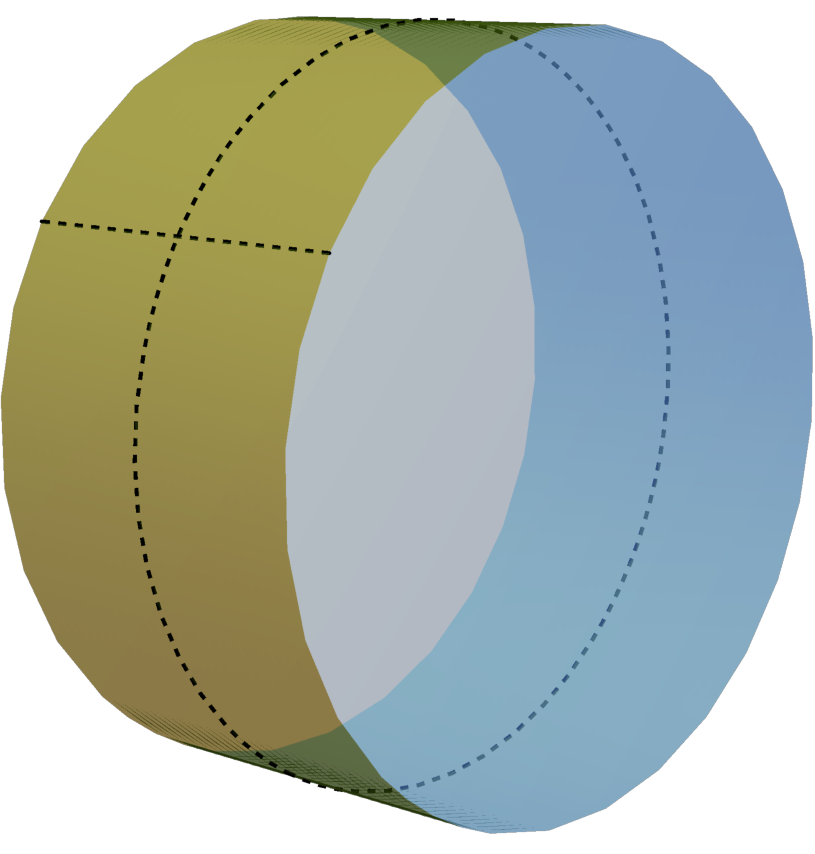
\includegraphics{Figures/Cilindro.pdf}
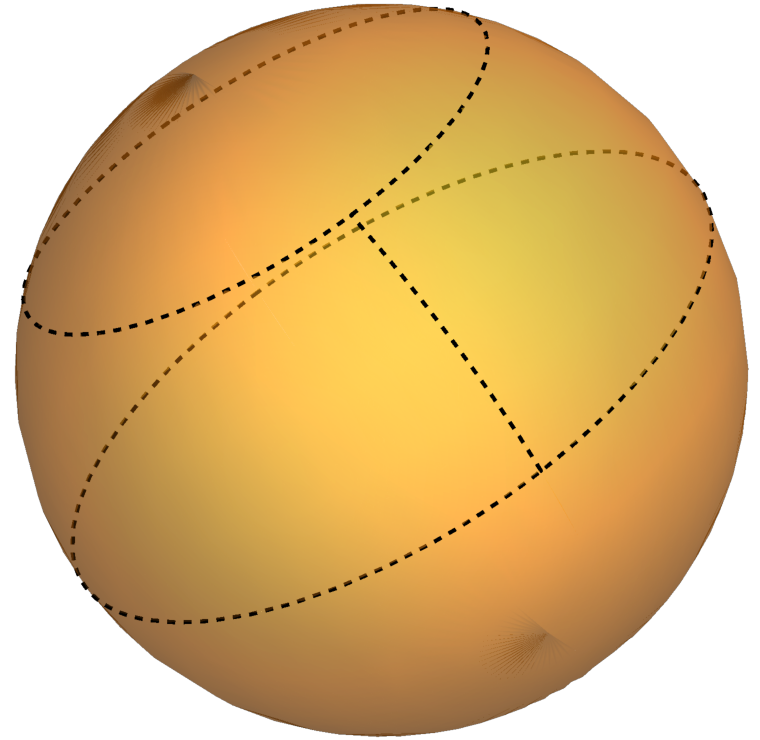
\includegraphics{Figures/Esfera.pdf}
\caption{Esfera y cilindro del \refexample{CilindroEsfera}. \labfig{Esfera}}
\end{marginfigure}

\begin{definition}
Sea $(X,A)$ un par de espacios. Tomando $C=S_*(X)$ y $D=S_*(A)$ en la
sucesión exacta (\ref{SECociente}), se obtiene la \textbf{sucesión exacta
asociada al par $(X,A)$}:
\[H_*(A) \xrightarrow{i_*} H_*(X) \xrightarrow{\pi_*} H_*(X,A)
\xrightarrow{\Delta} H_*(A)\]
\end{definition}

\begin{proposition}
$i_*$ es un isomorfismo si y sólo si $H_n(X,A)=0$ para todo $n \geq 0$.
\end{proposition}

Una \textbf{tríada de espacios} es una terna $(X,A,B)$, donde $(X,A)$ y
$(A,B)$ son pares de espacios.

Sea $(X,A,B)$ una tríada de espacios. Tomando $D=S_*(A)$, $E=S_*(B)$ y
$C=S_*(X)$ en \eqref{SECociente2}, se obtiene la sucesión exacta larga
\[H_n(A,B) \xrightarrow{i_*} H_n(X,B) \xrightarrow{j_*} H_n(X,A)
\xrightarrow{\Delta'} H_{n-1}(A,B)\]
donde $i_*$ y $j_*$ son los homomorfismos inducidos en homología por las
inclusiones $i\colon S_*(A) \hookrightarrow S_*(X)$ y $j\colon S_*(B)
\hookrightarrow S_*(A)$ y $\Delta'$ es la aplicación \eqref{DeltaCPrima}.

Recordemos que el grupo libre generado por el vacío es el grupo trivial, de
forma que $S_*(\emptyset)=0$. Esto nos permite establecer un isomorfismo
natural entre $S_*(X)$ y $S_*(X,\emptyset)$:
\begin{diag}
S_*(X) \arrow[r] & S_*(X,\emptyset)\\[-8mm]
c \arrow[r, maps to] & \overline c
\end{diag}
De la misma forma, se tiene que $S_*(X,A,\emptyset) \cong S_*(X,A)$ y
$S_*(X)\cong S_*(X,\emptyset,\emptyset)$.

\section{Aplicaciones entre pares}
\begin{definition}
Sean $(X,A)$ e $(Y,B)$ dos pares de espacios topológicos. Una
\textbf{aplicación de pares}
\[f\colon (X,A) \longrightarrow (Y,B)\]
es una aplicación continua $f\colon X \longrightarrow Y$ tal que $f(A)
\subseteq B$.
\end{definition}

Si $\phi\colon \sigma_p \to X$ es un símplice singular tal que
$\phi(\sigma_p) \subset A$ y $f\colon (X,A) \to (Y,B)$ es una
aplicación de pares, $(f\circ\phi)(\sigma_p) \subset B$, por lo que
$f_\#(\phi)$ es un $p$-símplice singular de $B$. Dado que la elección de
$\phi$ es arbitraria y los $p$-símplices singulares conforman una base de
$S_*(A)$,
\[f_\#(S_*(A)) \subseteq S_*(B)\]
por lo que $f$ induce una aplicación de cadenas
\begin{diag}
f_\#\colon S_*(X,A) \arrow[r] & S_*(Y,B)\\[-8mm]
\overline c \arrow[r, maps to] & \overline{f(c)}
\end{diag}
que induce a su vez un homomorfismo entre los grupos de homología relativa,
\begin{diag}
f_*\colon H_*(X,A) \arrow[r] & H_*(Y,B)\\[-8mm]
\left[\overline c\right] \arrow[r, maps to] & \left[\overline{f(c)}\right]
\end{diag}

Sean $f,g\colon (X,A) \to (Y,B)$ aplicaciones entre pares de espacios.
Decimos que $f$ es \textbf{homotópica} a $g$ si existe una aplicación entre
pares de espacios $F\colon (X\times I, A\times I) \to (Y,B)$ tal que
$F(x,0)=f(x)$ y $F(x,1)=g(x)$. Observar que $F$, al ser aplicación de pares,
se supone continua y verifica que $F(A\times I) \subset B$.

\begin{theorem}
Si $f,g\colon (X,A) \to (Y,B)$ son homotópicas como aplicaciones de pares,
\[f_*=g_*\colon H_*(X,A) \longrightarrow H_*(Y,B)\]
\end{theorem}

Tomando $A=\emptyset=B$, se obtiene el teorema de invarianza homotópica.

\begin{proof}
Sean $i_0,i_1\colon (X,A) \to (X\times I,A\times I)$ las aplicaciones
\begin{align*}
i_0(x)=(x,0); && i_1(x)=(x,1)
\end{align*}
Tenemos que $f=F\circ i_0$ y $g=F\circ i_1$. Para probar que $f_*=g_*$,
basta con probar que $(i_0)_\#$ e $(i_1)_\#$ son homotópicas como
aplicaciones de cadenas. La demostración es análoga al teorema de invarianza
homotópica.
\end{proof}

\begin{example}
Sean $X=[0,1]$, $Y=S_1 \subset \mb{R}^2$, $A=\{0,1\}$ y $B=\{(1,0)\}$.
Considérense las aplicaciones continuas $f,g\colon X \to Y$ definidas como
\begin{align*}
f(x)=e^{2\pi i x}; && g(x)=(1,0)
\end{align*}
Las aplicaciones $f$ y $g$ son homotópicas vía
\[F(x,t)=f(x)(1-t)+t\]
y además $f(A)=g(A)=B$, pero no forman una homotopía de pares entre $(X,A)$
e $(Y,B)$.
\end{example}

\subsection{Teorema de escisión}
\begin{lemma}[Lema de los cinco, \cite{FiveLemma}]
Sean $A_1,B_1,\dots,A_5,B_5$ grupos abelianos. Considérese el diagrama
conmutativo
\begin{diag}
A_1 \arrow{r} \arrow{d}{\alpha} & A_2 \arrow{r} \arrow{d}{\beta_1} &
A_3 \arrow{r} \arrow{d}{\gamma} & A_4 \arrow{r} \arrow{d}{\beta_2} &
A_5 \arrow{d}{\delta}\\
B_1 \arrow{r} & B_2 \arrow{r} & B_3 \arrow{r} & B_4 \arrow{r} & B_5
\end{diag}
cuyas filas forman sucesiones exactas. Si $\alpha$ es un epimorfismo,
$\beta_1$, $\beta_2$ son isomorfismos y $\delta$ es un monomorfismo,
$\gamma$ es un isomorfismo.
\end{lemma}

\begin{theorem}[Teorema de escisión]
Sea $(X,A)$ un par de espacios y $U \subset A$ tal que $\overline{U}
\subset \mathring A$. La aplicación inclusión $i\colon
(X\backslash U,A\backslash U) \hookrightarrow (X,A)$ induce un isomorfismo
\[i_*\colon H_*(X\backslash U,A\backslash U) \longrightarrow H_*(X,A)\]
\end{theorem}

\begin{marginfigure}
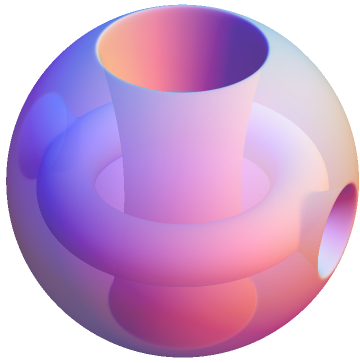
\includegraphics{Figures/HoleHoleHole.png}
\caption[Agujero en un agujero en un agujero]{El teorema de escisión nos dice
que la homología relativa de $X$ módulo $A$ sólo concierne a la frontera de
$A$. La estructura global del espacio no es relevante. Imagen: \cite{Hole}.}
\end{marginfigure}

\begin{proof}
Sea $\mc{U}=\{X\backslash U, \mathring A\}$. Tenemos por hipótesis que
\[(X\backslash U)^o=X\backslash\overline{U} \supset X\backslash\mathring{A}\]
por lo que $(X,\mc{U})$ es un espacio de Mayer-Vietoris. Si $\mc{U}'=
\{\mathring A,A\backslash U\}$, $(A,\mc{U}')$ también describe un espacio de
Mayer-Vietoris.

Los homomorfismos
\begin{align*}
i\colon S_*^\mc{U}(X) \hookrightarrow S_*(X);&&
i'\colon S_*^{\mc{U}'}(A) \hookrightarrow S_*(A)
\end{align*}
forman isomorfismos entre los grupos de homología. Teniendo en cuenta que
$S_*^{\mc{U}'}(A) \leq S_*^\mc{U}(X)$, la aplicación inclusión
\[j\colon S_*^{\mc{U},\mc{U}'}(X,A)=\frac{S_*^\mc{U}(X)}{S_*^{\mc{U}'}(A)}
\hookrightarrow \frac{S_*(X)}{S_*(A)}=S_*(X,A)\]
forma una aplicación de cadenas que da lugar al diagrama conmutativo
\begin{diag}
H_*(S_*^{\mc{U}'}(A)) \arrow{r} \arrow{d}{i'_*} &
H_*(S_*^\mc{U}) \arrow{r} \arrow{d}{i_*} &
H_*(S_*^{\mc{U},\mc{U}'}(X,A)) \arrow{r} \arrow{d}{j_*} &
H_*(S_*^{\mc{U}'}(A)) \arrow{d}{i_*}\\
H_*(A) \arrow{r} & H_*(X) \arrow{r} & H_*(X,A) \arrow{r} & H_*(A)
\end{diag}

\marginnote[-2.2cm]{
\begin{kaobox}[frametitle=Un detalle importante]
Dados tres grupos abelianos $A,B,C$ tales que $B+C \leq A+C$,
\[\frac{A+C}{B+C}\cong \frac{A}{B}\]
\end{kaobox}
}

Como $i_*$ e $i'_*$ son isomorfismos, el lema de los cinco nos garantiza que
$j_*$ es un isomorfismo, por lo que $S_*(X\backslash U,A\backslash U) \cong 
S_*^{\mc{U},\mc{U}'}(X,A)$ y concluimos que
\[H_*(X,A)\cong H_*(S_*^{\mc{U},\mc{U}'}(X,A)) \cong
H_*(X\backslash U,A\backslash U)\]
\end{proof}

\begin{example}\labexample{ToroAlambre}
\begin{enumerate}
\item Sea $X$ la esfera de la \reffig{Esfera}, $A$ el área
comprendida entre las dos circunferencias y $U\subset A$ una circunferencia
paralela a $\p A$. Tenemos que $X\backslash U$ son dos casquetes y
$A\backslash U$ son dos bandas. Ahora bien, observar que
\[\frac{X\backslash U}{A\backslash U} \cong \frac{X}{A}\]
por lo que ambos espacios tienen el mismo tipo de homología.
\item Sea $X$ el toro de Clifford,
\[A=\{[(x,y)] \in X\colon 1/4 \leq x \leq 3/4\}\]
y $\star \in A$. El subespacio $X\backslash\{\star\}$ es un toro
perforado. Podemos tomar el agujero y ensancharlo hasta quedarnos con dos
\emph{hilos de alambre} cruzados (que son los generadores de $H_1$). Esos
hilos forman una figura ocho.

Por otro lado, $A\backslash\{\star\}$ es un cilindro perforado. Podemos tomar
la perforación y ensancharla hasta quedarnos con las anillas de los bordes y
un alambre que los une. Dicho alambre se puede retraer hasta que las dos
anillas sean tangentes, formando una figura ocho.
\end{enumerate}
\end{example}

\begin{marginfigure}
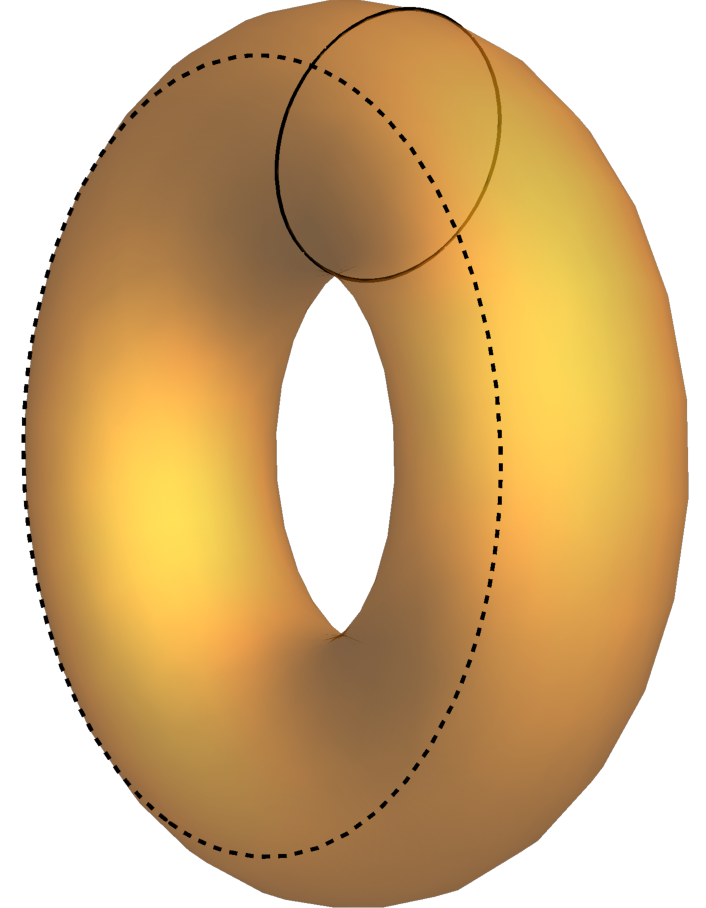
\includegraphics{Figures/ToroGeneradoresOrden1.pdf}
\caption{Generadores del grupo de homología de primer orden del toro.}
\end{marginfigure}

\section{Grupo de homología reducida}
Sea $X$ un espacio topológico. El camino constante
$\alpha\colon X \to \{\star\}$ da lugar a un homomorfismo en homologías
$\alpha_*\colon H_*(X) \to H_*(\{\star\})$. Se define el \textbf{grupo de
homología reducida} $\tilde H_*(X)$ como el núcleo de $\alpha_*$.

Si $X$ es convexo, sabemos por el \refthm{Convexo} que $H_n(X)=\{0\}$ para
todo $n > 0$, por lo que $\tilde H_n(X)=\{0\}$. Aún así, no podemos decir nada
del grupo de orden 0, porque $H_0(X)\cong \mb{Z}$.

La homología reducida está creada para poder describir de forma más sencilla
la homología de algunos espacios. Por ejemplo: todos los grupos de homología
reducida del espacio puntual son triviales, y el único grupo de homología
reducida no trivial de $S^n$ es el de orden $n$, como veremos más adelante.

En general, si un espacio es arcoconexo, su grupo de homología reducida de
orden cero es trivial.

\begin{proposition}
Sea $X$ un espacio topológico no vacío con una cantidad finita de
arcocomponentes. $\tilde{H}_0(X)$ es un grupo libre que verifica
\[\rk(\tilde{H}_0(X))=\rk(H_0(X))-1\]
\end{proposition}

\begin{proof}
Sea $c$ un $0$-ciclo de $X$. Si llamamos $X_1,\dots,X_n$ a las
arcocomponentes de $X$, existirán $a_1,\dots,a_n \in \mb{Z}$ tales que
\[c=\sum^n_{i=1}a_ix_i; \quad x_i \in X_i\]
Dado que $\alpha$ es una aplicación constante, podemos llamar $\alpha_0$ al
valor que toma en todos sus puntos, de forma que
\[0=\alpha_*([c])=\sum^n_{i=1}a_i[\alpha(x_i)]=[\alpha_0]\sum^n_{i=1}a_i\]

De aquí se deduce que $[c] \in \ker \alpha_*$ si y sólo si
\[a_n=-\sum^{n-1}_{i=1}a_i\]
por lo que $\{x_1,\dots,x_{n-1}\}$ forma un sistema generador libre de
$\tilde{H}_0(X)$. Por tanto,
\[\tilde{H}_0(X) \cong \mb{Z}^{n-1} \implies \rk(\tilde{H}_0(X))=
n-1=\mbox{rk }(H_0(X))-1\]
\end{proof}

Sea $f\colon X \to Y$ una aplicación continua. Al igual que $f$ induce un
homomorfismo entre grupos de homología, queremos ver que $f$ induce un
homomorfismo entre grupos de homología reducida. Para ello, sean $\alpha\colon
X \to \{\star\}$, $\beta\colon Y \to \{\star\}$ caminos constantes y $c=a_1x_1+
\dots+a_nx_n$ tal que $[c] \in \tilde H_n(X)$. Tenemos que
\[f_*([c])=\sum^n_{i=1}a_i[f(x_i)]=\sum^m_{j=1}b_j[y_j]\]
Dado que las aplicaciones continuas llevan conjuntos arcoconexos en conjuntos
arcoconexos,
\[\sum^n_{i=1}a_i=\sum^m_{j=1}b_j\]

Si $[c]$ está en $\ker \alpha_*$, la suma de todos los $a_i$ es 0. Como la
suma de los $a_i$ es la misma que la de los $b_j$, esto es tanto como decir
que $f_*([c])$ está en $\ker \beta_*$. Por tanto, $f_*(\ker \alpha_*) \leq
\ker \beta_*$, de forma que $f$ induce un homomorfismo entre los grupos de
homología reducida de $X$ e $Y$.

\begin{example}
Si $X$ es un espacio contráctil, $\tilde{H}_*(X)=0$.
\end{example}

\subsection{Una fórmula para la homología reducida}
\begin{lemma}[Lema de escisión]
Sean $A,B,C$ grupos abelianos. Considérese la sucesión exacta corta
\[0 \longrightarrow A \xrightarrow{f} B \xrightarrow{g} C \longrightarrow 0\]
Las siguientes afirmaciones son equivalentes:
\begin{enumerate}
\item $B$ es suma directa de $A$ con $C$;
\item existe un homomorfismo $h\colon B \to A$ tal que $f\circ h=\id_A$;
\item existe un homomorfismo $k\colon C \to B$ tal que $k\circ g=\id_C$.
\end{enumerate}
\end{lemma}

\begin{proposition}\labprop{ReducidoRelativo}
Dado un $p \in X$,
\[\tilde{H}_*(X)\cong H_*(X,\{p\})\]
\end{proposition}

\begin{proof}
Sea $i\colon \{p\} \hookrightarrow X$ la inclusión. La aplicación continua
\[\alpha: X \longrightarrow {p}\]
verifica que $\id_{\{p\}}=\alpha\circ i$, por lo que $\{p\}$ forma un
retracto de $X$ e $i_*$ es un monomorfismo.

Considérere la sucesión exacta de homología generada por el par de espacios
$(X,\{p\})$:
\[H_n(\{p\}) \xrightarrow{i_*} H_n(X) \xrightarrow{j_*}
H_n(X,\{p\}) \xrightarrow{\Delta'} H_{n-1}(\{p\})\]
Como $i_*$ es un monomorfismo, $\im \Delta'=\ker i_*=0$. Por el primer teorema
de isomorfia, $\im j_*=\ker \Delta'=H_n(X,p)$, por lo que $j_*$ es sobreyectiva.

Dado que $i_*$ es inyectiva y $j_*$ es sobreyectiva, podemos pasar a definir
una sucesión exacta corta en lugar de trabajar con una sucesión exacta
larga:
\[0 \longrightarrow H_n(\{p\}) \xrightarrow{i_*} H_n(X) \xrightarrow{j_*}
H_n(X,\{p\}) \longrightarrow 0\]

Sabemos que $\alpha_* \circ i_*=\id_{H_*(\{p\})}$, por lo que el lema de
escisión nos garantiza que existe un homomorfismo
\[\beta\colon H_n(X,\{p\}) \to H_n(X)\]
tal que $j_*\circ \beta=\id_{H_n(X,\{p\})}$. Esto es tanto como decir que
$\beta$ es inyectiva.

Se puede probar que $\im \beta=\ker \alpha_*=\tilde{H}_*(X)$, por lo que
hemos hallado un isomorfismo entre $H_*(X,\{p\})$ y $\tilde{H}_*(X)$.
\end{proof}

Sea $X$ un espacio topológico con $n$ componentes arcoconexas. Hasta ahora,
sabemos que
\[\tilde H_0(X) \cong \mb{Z}^{n-1}\]
pero queda pregunta preguntarnos qué ocurre con los grupos de orden
superior. Utilizando la \refprop{ReducidoRelativo}, tenemos para cada $p > 0$ y
el espacio puntual $\star$ que
\[\tilde{H}_p(X)\cong H_p(X,\star)=\frac{Z_p(X,\star)}{B_p(X,\star)}=
\frac{Z_p(X)/Z_p(\star)}{B_p(X)/B_p(\star)}\]
Teniendo en cuenta que $Z_p(\star)=B_p(\star)$, estamos en condiciones de
aplicar el tercer teorema de isomorfia:
\[\tilde{H}_p(X)\cong \frac{Z_p(X)/Z_p(\star)}{B_p(X)/B_p(\star)}=
\frac{Z_p(X)/B_p(\star)}{B_p(X)/B_p(\star)} \cong
\frac{Z_p(X)}{B_p(X)}=H_p(X)\]

De esta forma, llegamos a que el grupo de homología reducida sólo
\textit{reduce} el grupo de orden cero, cuya única función es contar el
número de componentes conexas.

\begin{corollary}\label{HomoReducida}
Sea $X$ un espacio topológico con una cantidad finita de arcocomponentes.
\[\tilde{H}_*(X)\cong \frac{H_*(X)}{H_*(\star)}\]
\end{corollary}

\begin{example}
$$\tilde{H}_*(B_p)\cong\frac{H_*(B_p)}{H_*(\star)}\cong
\begin{cases}\mb{Z}^p & \mbox{ si } n=1\\0 & \mbox{ si no}\end{cases}$$
\end{example}

\subsection{Homología reducida y homología relativa}
En lo sucesivo, diremos que un espacio topológico es de \textbf{tipo $C_2$}
si es compacto y $T_2$ al mismo tiempo.

\marginnote[-2.2cm]{
\begin{kaobox}[frametitle=Idea de la demostración]
En el lema, nos proporcionan una aplicación cociente $\pi$ que
envía $X$ en $X_A$ de forma continua, por lo que nuestro impulso inicial
sería definir
\[G=\pi \circ F \circ (\pi \times \id_I)^{-1}\]
El problema es que $\pi^{-1}$ no está bien definido, por lo que tampoco lo va
a estar $(\pi\times \id_I)^{-1}$. Lo que haremos será definir una $G$ tal que
\[G\circ \pi=(\pi\circ\id_I)\circ F\]
\end{kaobox}
}

\begin{lemma}\label{RetrCoci}
Sea $(X,A)$ un par de espacios donde $X$ es $C_2$ y $A$ es cerrado en $X$.
Considérese la aplicación cociente
\[\pi\colon X \to \frac{X}{A}\]
y sea $y=\pi(A) \in X/A$. Si $A$ es retracto por deformación fuerte de $X$,
$\{y\}$ es un retracto por deformación fuerte de $\pi(X)=X/A$.
\end{lemma}

\begin{proof}
Dado que $A$ es un retracto por deformación fuerte de $X$, existe una
homotopía $F\colon X \times I \to X$ tal que $F(x,0)=x$ para todo $x \in X$,
$F(a,t)=a$ para todo $a \in A$ y $t \in I$, y $F(X\times\{1\}) \subseteq A$.

Si $X_A=X/A$, queremos hallar una homotopía $G\colon X_A\times I \to X_A$ tal
que $G([x],0)=x$ para todo $x \in X_A$, $G(X_A\times\{1\})=\{y\}$ y $G(y,t)=y$
para todo $t \in I$.

Sea $G\colon X_A\times I \longrightarrow X_A$ la aplicación
\[G([x],t)=(\pi\circ F)(x,t)\]
Si $x \not\in A$, la clase de $x$ módulo $A$ es el singulete formado por el
propio punto $x$, por lo que $G$ está bien definido en $X_A\backslash\{y\}$.

Si $x \in A$, sabemos que $F(a,t)=a$ para todo $t \in I$, por lo que
\[(\pi\circ F)(a,t)=\pi(a) \in \pi(A)=\{y\}\]
De esta forma, $G$ está bien definida y que $G(y,t)=y$ para todo $t \in I$.

Sea $p \in X/A$. Si $x \in \pi^{-1}(p)$, sabemos que $F(x,0)=x$, por lo que
\begin{align*}
G(p,0)&=(\pi\circ F)(x,0)=\pi(x)=p\\
G(p,1)&=(\pi \circ F)(x,1)\in \pi(A)=\{y\}
\end{align*}

\marginnote[-2.2cm]{
\begin{kaobox}[frametitle=Detalles de la prueba]
\begin{itemize}
\item Una aplicación es continua si y sólo si la preimagen de todo cerrado es
cerrada.
\item Los subespacios cerrados de un compacto son compactos.
\item La imagen de un compacto por una aplicación continua es compacta.
\item Todo subespacio compacto de un espacio de Hausdorff es cerrado.
\end{itemize}
\end{kaobox}
}
Sólo nos queda ver que $G$ es continua. Para ello, sea $C$ un subconjunto
cerrado de $X/A$. Por continuidad, $D=(\pi\circ F)^{-1}(C)$ es un subconjunto
cerrado de $X\times I$. Como $X\times I$ es compacto, $D$ es compacto. Por
continuidad, $(\pi\times \id_I)(D)$ es compacto. Por cómo se define $G$,
\[G^{-1}(C)=(\pi\times 1_I)(D) \subseteq X_A \times I\]
es compacto. Dado que
$X_A\times I$ es un espacio de Hausdorff, $G^{-1}(C)$ es cerrado.

Dado que la elección de $C$ es arbitraria, se sigue que $G$ es continua.
\end{proof}

\begin{lemma}
Sea $X$ un espacio $C_2$. Dados dos cerrados disjuntos $C,D \subset X$,
existen abiertos $U,V \subset X$ tales que $U$ contiene a $C$, $V$ contiene
a $D$ y $U\cap V=\emptyset$
\end{lemma}

\begin{proof}
Dados $x \in C$ e $y \in D$, como $C$ y $D$ son disjuntos, $x \neq y$. Como
$X$ es un espacio de Hausdorff, existen $U_y$, $V_y$ abiertos tales que
\begin{align*}
x \in U_y; && y \in V_y; && U_y\cap V_y=\emptyset
\end{align*}
Como $D$ es un subespacio cerrado de un compacto, $D$ es compacto, por lo
que podemos hallar una familia finita de puntos $y_1,\dots,y_n \in D$ tales
que $\{V_{y_1},\dots, V_{y_n}\}$ forma un recubrimiento abierto de $D$.

Para cada $i \in \{1,\dots,n\}$, podemos hallar un abierto $U_i \subseteq X$
tal que $U_i\cap V_{y_i}=\emptyset$ y $x \in U_i$. Se  definen entonces
\begin{align*}
U_x=\bigcup_{i=1}^nU_i;&&  V_x=\bigcup_{i=1}^n V_{y_i}
\end{align*}
Notar que ambos conjuntos son abiertos y $U_x\cap V_x=\emptyset$.

Dado que $C$ es un subespacio cerrado de un compacto, $C$ es compacto, por
lo que podemos hallar una familia finita de puntos $x_1,\dots,x_n$ tales que
$\{U_{x_1},\dots,U_{x_m}\}$ forma un recubrimiento abierto de $C$.

Para terminar, considérense los abiertos
\begin{align*}
U=\bigcup _{i=1}^m U_{x_i};&&  V=\bigcup_{i=1}^m V_{x_i}
\end{align*}
Se tiene por construcción que $D \subseteq V$ y $U\cap V=\emptyset$.
\end{proof}

\begin{lemma}\lablemma{LemaB}
Sea $X$ un espacio $C_2$. Dado un cerrado $A$ contenido en un abierto $V$,
existe un abierto $W$ tal que
$$A \subseteq W \subseteq \overline{W} \subseteq V$$
\end{lemma}

\begin{proof}
Considérense los cerrados $A$ y $X\backslash V$. Por el lema anterior, existen
abiertos $U,W$ de $X$ tales que $A \subseteq W$, $X\backslash V \subseteq U$ y
$U\cap W=\emptyset$. Tenemos que $U\cap W=\emptyset$, por lo que
\[W \subseteq X\backslash U \subseteq V \implies
\overline{W} \subset \overline{X\backslash U}=X\backslash U \subseteq V\]
\end{proof}

\begin{theorem}[Teorema del retracto]\labthm{Retracto}
Sea $X$ un espacio $C_2$, $A$ un subespacio cerrado de $X$ y $\pi\colon (X,A)
\to (X/A,\pi(A))$ una aplicación cociente. Si $A$ es un retracto por
deformación fuerte de algún entorno cerrado de $A$ en $X$,
\[H_*(X,A) \cong H_*(X/A,\pi(A)) \cong \tilde{H}_*(X/A)\]
\end{theorem}

\begin{proof}
Considérese la sucesión exacta asociada a la tríada de espacios $(X,U,A)$:
\[H_*(U,A) \xrightarrow{i_*} H_*(X,A) \xrightarrow{j_*} H_*(X,U)
\xrightarrow{\Delta'} H_*(U,A)\]
Dado que $A$ es un retracto por deformación fuerte de $U$, $H_*(U,A)=0$. Por
exactitud, se sigue que $0=\im i_*=\ker j_*$ y $\im j_*=\ker \Delta'=
H_*(X,U)$. Por tanto,
\[H_*(X,A) \cong H_*(X,U)\]

Sabemos que $X$ es un espacio $C_2$ y que $A$ es cerrado. Como $U$ es
entorno de $A$, $A \subseteq \mathring U$. Usando el \reflemma{LemaB}, podemos
hallar un abierto $V \subseteq X$ tal que $A \subseteq V \subseteq
\overline{V} \subseteq \mathring U \subseteq U$. Aplicando el teorema de
escisión, la inclusión $i\colon (X\backslash V,U\backslash V) \hookrightarrow
(X,U)$ induce un isomorfismo $i_*$. Se sigue que
\[H_*(X,U)\cong H_*(X\backslash V,U\backslash V)\]

Considérese la aplicación $p=\pi|_{X\backslash V}$. Como $A \subseteq V$,
$\pi(x)$ sólo tiene un representante (el propio $x$), de forma que $p$ es un
homeomorfismo. Como $\pi(U\backslash V)=\pi(U)\backslash \pi(V)$, se sigue que
\[H_*(X\backslash V,U\backslash V)\cong
H_*(X_A\backslash \pi(V),\pi(U)\backslash \pi(V))\]

Aplicando el teorema de escisión al par $(X_A,\pi(U))$, se obtiene el
isomorfismo
\[H_*(X_A\backslash \pi(V),\pi(U)\backslash \pi(V)) \cong H_*(X_A,\pi(U))\]

Considérese la sucesión exacta asociada a la tríada de espacios\\
$(X_A,\pi(U),\pi(A))$. Un procedimiento similar al que hemos desarrollado al
inicio de la demostración nos lleva a concluir que
\[H_*(X_A,\pi(U))\cong H_*(X_A,\pi(A))\]
\end{proof}

\section{Homeomorfismo relativo}
\begin{definition}
Un \textbf{homeomorfismo relativo} es una aplicación continua entre pares de
espacios $f\colon (X,A) \to (Y,B)$ tal que
\[f\colon X\backslash A \longrightarrow Y\backslash B\]
es un homeomorfismo.
\end{definition}

\begin{example}
\begin{enumerate}
\item Si $\mc{N}=(0,0,1) \in S^2$ y $D^2$ denota a la bola cerrada unidad de
$\mb{R}^2$, existe un homeomorfismo
\[f\colon D^2\backslash \partial D^2 \longrightarrow S^2\backslash\{\mc{N}\}\]
De esta forma, $f$ induce un homeomorfismo relativo entre los pares 
$(S^2,\{\mc{N}\})$ y $(D^2,\partial D^2)$.
\item Si $C=S^1\times I$ es un cilindro y $\mc{S}=(0,0,-1) \in S^2$, existe un
homeomorfismo
\[g\colon S^1\times \mathring{I} \to S^2-\{\mc{N},\mc{S}\}\]
que identifica al cilindro sin anillas con $S^2$
\end{enumerate}
\end{example}

\begin{theorem}[Teorema del homeomorfismo relativo]\labthm{HomeoRelativo}
Sean $X$, $Y$ espacios $C_2$, $A \subseteq X$ y $B \subseteq Y$ cerrados y
$f\colon (X,A) \to (Y,B)$ un homeomorfismo relativo. Si $A$ es retracto por
deformación fuerte de algún entorno compacto de $A$ en $X$ y $B$ es retracto
por deformación fuerte de algún entorno compacto de $B$  en $Y$, $f_*$ es un
isomorfismo.
\end{theorem}

\begin{proof}
Sean $\pi\colon X \to X/A$ y $\pi'\colon Y \to Y/B$ aplicaciones cociente. Se
define la aplicación $f'\colon X/A \to Y/B$ como $f([x])=\pi'(f(x))$.
Es fácil ver que $f'$ está bien definida y es continua, por lo que da lugar
al siguiente diagrama conmutativo:
\begin{diag}
X \arrow{r}{f} \arrow{d}{\pi} & Y \arrow{d}{\pi'}\\
X/A \arrow{r}{f'} & Y/B
\end{diag}

Dado que $f$ es un homeomorfismo relativo, $f'$ es una biyección entre $X/A$
e $Y/B$. Como ambos son espacios $C_2$, $f'$ es un homeomorfismo, por lo que
induce un isomorfismo entre $H_*(X/A)$ y $H_*(Y/B)$.

Tenemos entonces el diagrama conmutativo
\begin{diag}
H_*(X,A) \arrow{r}{f_*} \arrow{d}{\pi_*} & H_*(Y,B) \arrow{d}{\pi'_*}\\
H_*(X/A,\pi(A)) \arrow{r}{f'_*} & H_*(Y/B,\pi'(B))
\end{diag}

Sabemos por el \refthm{Retracto} que $\pi'_*$ y $\pi_*$ son isomorfismos;
además, acabamos de probar que $f_*'$ es un isomorfismo. Como consecuencia,
$f_*$ es un isomorfismo.
\end{proof}
